\section{Full-record reproduction and learned-partial diagnostics}
\label{sec:reproduction_audit}

\subsection{Historical records versus new executions}
The original all-seed archives named in \texttt{docs/DATA\_MANIFEST.json}
could not be located. Their recorded checksums do not make them available.
The repository did retain every original structured-study and paired-transfer
summary, along with the ten structured-study and two transfer traces for seed~10.
We therefore executed the unchanged declared protocols again, preserving
the historical records and using separate output directories. These are
newly reproduced simulation records, not recovered original archives.
The historical reconstruction status of contact and Burgers is unchanged.

The reproduction uses an immutable snapshot of the simulation sources and
configurations from repository commit
\texttt{374187a31d69e9c93eded1bbc8440696804364b9}.
Source hashes were checked against that commit before comparing outcomes.
The runner records the invocation, all seeds, configurations, package
versions, platform, random-generator identity and states, per-run status,
and file hashes. Two worker processes and one numerical-library thread per
worker were used. The execution environment is Python~3.12.3,
NumPy~2.3.5, SciPy~1.17.0, and Matplotlib~3.10.8; the historical metadata
records Python~3.13.5. Thus identical environment provenance is not claimed.

All 120 declared runs completed, with no failed or excluded seeds:
100 original structured-study runs and 20 paired-transfer runs. The independent audit
passed 7,851 checks. Every regenerated per-run summary and the main and
transfer aggregate tables matched their saved historical counterparts
numerically; the maximum absolute difference was zero. All twelve
previously available raw-run arrays also matched numerically with
maximum absolute difference zero. These agreements do not establish
byte identity with either missing historical ZIP, whose original
contents were unavailable. No historical record or value was overwritten;
the retained normalized periodic-plant experiment has separately identified records.


The audit recomputes task errors, evaluated partials, compatibility
energies, aggregation windows, sample standard deviations, saturation,
and frozen-model checks from the generated records. Contact integral
energies and Fourier complete-feature energies are additionally
reconstructed from their declared sensor-noise streams. Existing
overwrite-prone summarization scripts are not invoked. Comparisons use
relative tolerance $10^{-9}$ and absolute tolerance $10^{-11}$;
the reported maximum differences describe the actual observations, not
merely acceptance within tolerance.

The original scripts record time-step diagnostics and selected partial or
field snapshots, rather than every noisy sensor vector. For example,
Burgers field snapshots are spaced by $0.1$~s. The retained executable
source, configurations, seeds, and PCG64 generator states specify how to
regenerate the full sensing sequence. The new estimator comparison also
saves its observed rate stream explicitly. This distinction prevents
calling a diagnostic trace a complete original sensor log.

Separate regenerated structured-study and excitation archives contain source,
configuration, execution, audit, and checksum evidence with their records.
Their names and hashes are recorded in
\texttt{docs/REPRODUCTION\_20261118.json}; the old archive manifest is
preserved. These are local artifacts at this revision, not an asserted
public release or permanent data deposit. New comparison and direct-lift
records have separate protocol identities and do not overwrite any historical
statistic. Their local archive is described in
\path{docs/SUPPLEMENTARY_STUDIES_20261118.json}, including the comparison,
both direct-learning studies, and learned-partial postprocessing.
The retained normalized periodic-plant Fourier experiment has its own records and archive,
described in Section~\ref{sec:normalized_fourier_results} and
\path{docs/NORMALIZED_FOURIER_20261118.json}. The current direct-field
main experiments have separate identities and records in
Section~\ref{sec:direct_main}.

\subsection{Errors on coefficient-dependent partial entries}
The full-matrix error used in the original experiments includes supplied
derivative entries in its denominator. To distinguish estimation from
correct supplied structure, we also evaluate $e_{F,U}$ in
(\ref{eq:audit_unknown_only}) on every reproduced run. Contact excludes
the supplied $\rho$, unit and fixed-zero entries; Fourier excludes the
input partial $-1$; Burgers excludes the unit $w_t$ partial. The original
context and row scalings are retained. All remaining true denominators
are nonzero in these records, and supplied blocks were checked to be
identical between the estimated and true matrices. ``Learned entries'' in
the retained diagnostic labels means coefficient-dependent evaluated
entries; it does not mean that those entries were independent learner
states. Excluding supplied entries from a metric changes its denominator,
not the underlying learning rule.

\begin{table*}[t]
\centering
\caption{Reproduced original protocols: late-window evaluated-partial
errors, mean $\pm$ sample standard deviation across all ten seeds.
Contact uses $[100,120)$~s, Fourier $[60,80)$~s, and Burgers $[18,24)$~s.
Contact and Burgers use saved $0.1$-s partial snapshots; Fourier uses all
$0.01$-s records. Consequently snapshot averages need not equal the
original all-step means. Different physical scalings prevent interpreting
the rows as a comparison of difficulty across systems.}
\label{tab:unknown_partials}
\begin{tabular}{llcc}
\toprule Study & Method & All entries & Learned entries \\
\midrule
Contact & learned & $0.000896\pm0.00043$ & $0.000915\pm0.00044$ \\
Contact & frozen & $0.584\pm7.8\times10^{-7}$ & $0.596\pm7.5\times10^{-7}$ \\
Contact & oracle & $0\pm0$ & $0\pm0$ \\
Fourier & learned & $0.00687\pm0.00019$ & $0.00855\pm0.00023$ \\
Fourier & K0 & $0.185\pm8.6\times10^{-6}$ & $0.224\pm1\times10^{-5}$ \\
Fourier & frozen & $0.214\pm2.9\times10^{-17}$ & $0.26\pm5.9\times10^{-17}$ \\
Fourier & oracle & $0\pm0$ & $0\pm0$ \\
Burgers & learned & $0.000108\pm9.7\times10^{-6}$ & $0.000147\pm1.3\times10^{-5}$ \\
Burgers & frozen & $0.159\pm0$ & $0.217\pm0$ \\
Burgers & oracle & $0\pm0$ & $0\pm0$ \\
\bottomrule
\end{tabular}

\end{table*}

\begin{figure*}[t]
\centering
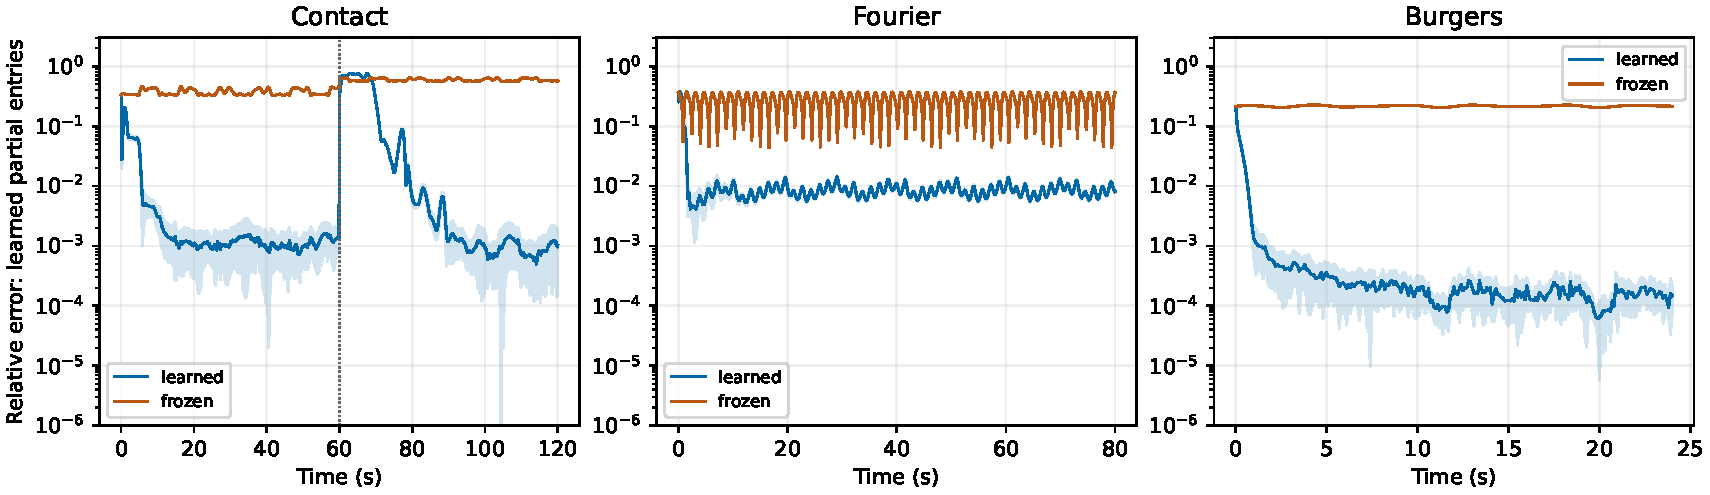
\includegraphics[width=.98\textwidth]{unknown_partial_tracking.pdf}
\caption{Original structured protocols: error restricted to learned partial entries on each controller's
own trajectory. Lines are ten-seed means and shading is one sample
standard deviation; no temporal smoothing is applied. The contact change
occurs at $60$~s. The logarithmic display range does not modify recorded
errors; exact oracle curves are omitted from this plot and retained in
Table~\ref{tab:unknown_partials}. The Fourier panel uses the bounded
six-coefficient protocol, distinct from both the retained normalized
periodic-plant study and the current direct-field main benchmark.}
\label{fig:unknown_partial_tracking}
\end{figure*}

These diagnostics directly test the evaluated derivatives on the observed
contexts, including contact recovery after changed material and actuation
and the varying Fourier phase column. They do not turn a prescribed-family
fit into unrestricted Jacobian discovery. The stationary Fourier
coefficients can generate rapidly changing derivatives, whereas contact
requires the coefficients themselves to adapt after the change. Both
effects should be distinguished from optimization progress alone.
The online data remain dependent on the controller and prior updates;
frozen transfer and evaluator-only query tests in Section~\ref{sec:excitation}
address a separate, narrower form of reuse.
